% THIS DOCUMENT IS FOLLOWS THE VOLERE TEMPLATE BY Suzanne Robertson and James Robertson
% ONLY THE SECTION HEADINGS ARE PROVIDED
%
% Initial draft from https://github.com/Dieblich/volere
%
% Risks are removed because they are covered by the Hazard Analysis
\documentclass[12pt]{article}

\usepackage{graphicx} 
\graphicspath{ {./res/} }
\usepackage{booktabs}
\usepackage{tabularx}
\usepackage{longtable}
\usepackage{graphicx}
\usepackage{hyperref}
\usepackage{float}
\graphicspath{ {./res/} }
\usepackage{amsmath, mathtools}
\usepackage{pdflscape}
\usepackage{multirow}
\hypersetup{
    bookmarks=true,         % show bookmarks bar?
      colorlinks=true,      % false: boxed links; true: colored links
    linkcolor=red,          % color of internal links (change box color with linkbordercolor)
    citecolor=green,        % color of links to bibliography
    filecolor=magenta,      % color of file links
    urlcolor=cyan           % color of external links
}

\newcommand{\lips}{\textit{Insert your content here.}}

%% Comments

\usepackage{color}

\newif\ifcomments\commentstrue %displays comments
%\newif\ifcomments\commentsfalse %so that comments do not display

\ifcomments
\newcommand{\authornote}[3]{\textcolor{#1}{[#3 ---#2]}}
\newcommand{\todo}[1]{\textcolor{red}{[TODO: #1]}}
\else
\newcommand{\authornote}[3]{}
\newcommand{\todo}[1]{}
\fi

\newcommand{\wss}[1]{\authornote{blue}{SS}{#1}} 
\newcommand{\plt}[1]{\authornote{magenta}{TPLT}{#1}} %For explanation of the template
\newcommand{\an}[1]{\authornote{cyan}{Author}{#1}}

%% Common Parts

\newcommand{\progname}{ProgName} % PUT YOUR PROGRAM NAME HERE
\newcommand{\authname}{Team \#, Team Name
\\ Student 1 name
\\ Student 2 name
\\ Student 3 name
\\ Student 4 name} % AUTHOR NAMES                  

\usepackage{hyperref}
    \hypersetup{colorlinks=true, linkcolor=blue, citecolor=blue, filecolor=blue,
                urlcolor=blue, unicode=false}
    \urlstyle{same}
                                


\begin{document}

\title{Software Requirements Specification for \progname: An application to help users save on grocery spending.} 
\author{\authname}
\date{\today}
	
\maketitle

~\newpage

\pagenumbering{roman}

\tableofcontents

~\newpage

\section*{Revision History}

\begin{tabularx}{\textwidth}{p{3cm}p{2cm}X}
\toprule {\textbf{Date}} & {\textbf{Version}} & {\textbf{Notes}}\\
\midrule
06/10/23 & 1.0 & Initial version of the SRS\\
\bottomrule
\end{tabularx}

~\\

~\newpage
\section{Purpose of the Project}

This section will go cover the reason for creating this project by going over the user business and application as well
as its goals.

\subsection{User Business}

With the world currently facing record high inflation, cost-of-living is among the highest
it has ever been. This affects all daily necessities but is especially true for food and groceries.
According to Statistics Canada, cost of groceries between March and April 2023 were 20\% higher than they were
two years ago [1]. More recently, grocery inflation was at 5.4\% year-over-year in October indicating how groceries
are only continuing to increase in price [2].
As a whole, all households are affected but there is particular financial strain on those with lower-incomes.
As a result, interest in personal finance has grown and become more important in peoples' everyday lives.
To assist these individuals, we are developing an application that can help users better understand their
spending habits and make smarter financial decisions. This application will allow users to
take photos of grocery receipts and track their overall spending, analyze spending trends, and receive
suggestions on cheaper alternatives for purchased grocery items. Overall, we believe this application
will help users stay more informed and reduce grocery spending in the long-term.

\subsection{Goals of the Project}
\begin{itemize}
  \item The created application will help users save money on groceries over time.
  \item The application will provide accurate spending data and suggestions to end users.
\end{itemize}  
\section{Stakeholders}
\subsection{Client}
Both the client and customer will be the users of the system. These primary stakeholders are made up of low-income households of Hamilton and university students from McMaster who want to save money on groceries. The stakeholders will make decisions that influence the system through surveys, studies, and focus groups.
\subsection{Customer}
Outlined in the above Client section.
\subsection{Other Stakeholders}
\begin{itemize}
  \item Grocery stores in the area
  \item Household members (people who the groceries are being purchased for)
  \item Mobile application stores (iOS app store, Google Play Store)
  \item Any individuals who wants to save on groceries
\end{itemize}

\subsection{Hands-On Users of the Project}
Low income households and individuals who are budget constrained on their groceries. The archetypal customer will have access to a device with a camera and have access to the internet. This entails adults or young adults who are responsible for making decisions on grocery items. Customers want to reduce the cost of their grocery items whilst maximizing the convenience of their grocery shopping trip. 
\begin{itemize}
  \item Low or single income households in Hamilton
  \begin{itemize}
    \item Shops for household groceries.
    \item Moderate experience with navigation mobile applications.
    \item 30-70 years of age.
    \item Has vehicle or some means to travel.
  \end{itemize}
  \item Students of McMaster University
  \begin{itemize}
    \item Shops for individual groceries
    \item Adept experience with navigation mobile applications.
    \item 20-30 years of age.
    \item Has no vehicle or limited means to travel.
  \end{itemize}
\end{itemize}

\subsection{Personas}
\begin{itemize}
  \item John Bertuzzi
  \begin{itemize}
    \item Age: 22
    \item Favorite food: Chicken and Pasta
    \item Nursing Student at McMaster University
    \item Living in Ainslie Wood East.
    \item Athlete.
    \item Missing teeth.
  \end{itemize}
  \item Alice Woll
  \begin{itemize}
    \item Age: 51
    \item Favorite food: Grilled Cheese
    \item Mother of 2, Spouse of William Woll.
    \item Accountant for tech company.
    \item Living in Westdale.
    \item Likes to watch Hockey.
  \end{itemize}
\end{itemize}

\subsection{Priorities Assigned to Users}
All users will have equal priority within the system.

\subsection{User Participation}
Everyday users will provide their shopping data to the community database. This will be of no additional time commitment than they are already required to use the system at a base level.

From an elicitation perspective, a sample of users will be responsible for providing usability, look, and feel requirements feedback. This will be done at various stages in development.
\subsection{Maintenance Users and Service Technicians}
N/A

\section{Mandated Constraints}
\subsection{Solution Constraints}
\textbf{Mobile Device}\\
\underline{Description}: User will interact with the system through an app on their mobile device (smartphone).\\
\underline{Rationale}: Mobile devices are widely used and ubiquitous. While at a grocery store, users may need access to the system.\\
\underline{Fit Criterion}: User interface will run entirely on a mobile device.\\
\\
\textbf{Internet Access}\\ %%todo: is this too solution specific?
\underline{Description}: User must have internet access.\\
\underline{Rationale}: System servers and databases are used to store collective user data and process that data. User's devices are required to communicate with the servers and databases via internet access.\\
\underline{Fit Criterion}: User interface will have internet access.\\
\\
\textbf{Device with Camera}\\
\underline{Description}: User must be equipped with a device that has a camera. This should be quite common as most smartphones have a camera.\\
\underline{Rationale}: Users will be using the system while they are out on their grocery trips. Thus, the system needs to have a quick and easy method of data input. This also makes it easier for those who have their hands full or do not have the finger mobility to effectively type on their phone keyboards.\\
\underline{Fit Criterion}: System must have access to a mobile camera.\\

\subsection{Implementation Environment of the Current System}
\begin{figure}[H]
  \centering
  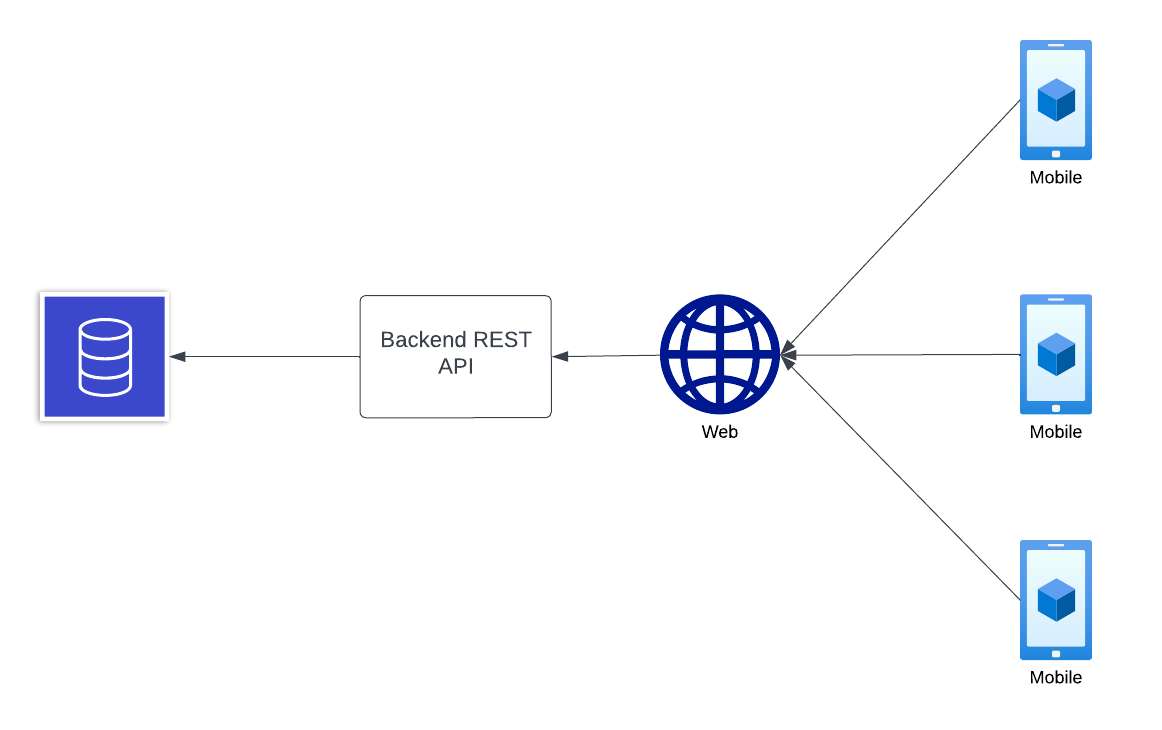
\includegraphics[width=\textwidth]{ImplementationEnvironment.png}
  \caption{Implementation Environment}
  \label{fig:ImplementationEnvironment}
\end{figure}

\subsection{Partner or Collaborative Applications}
N/A
\subsection{Off-the-Shelf Software}
The system requires the following off-the-shelf software:
\begin{itemize}
  \item \href{https://github.com/tesseract-ocr/tesseract}{Tesseract} OCR.
  \item \href{https://flutter.dev/}{Flutter} for Front-end.
  \item \href{https://nodejs.org/en}{NodeJS} for Back-end.
  \item \href{https://www.npmjs.com/package/express}{Express} REST API.
  \item \href{https://www.postgresql.org/}{PostgreSQL} as Relational Database.
\end{itemize}

\subsection{Anticipated Workplace Environment}
N/A
\subsection{Schedule Constraints}
The schedule for this project is in adherance with the milestones implemented by our course instructor. Found \href{https://gitlab.cas.mcmaster.ca/courses/capstone/-/blob/main/CourseOutline/Capstone_Outline.pdf}{here}.
\subsection{Budget Constraints}
The project budget is \$750 paid for directly by the developers.
\subsection{Enterprise Constraints}
N/A
\section{Naming Conventions and Terminology}
\subsection{Glossary of All Terms, Including Acronyms, Used by Stakeholders
involved in the Project}
\begin{table}[htbp]
    \centering
    \begin{tabularx}{\textwidth}{|>{\hsize=.4\hsize}X|>{\hsize=1.6\hsize}X|}
        \hline
        \textbf{Term} & \textbf{Definition}\\
        \hline
        Consumer & A person who purchases goods and is a user of our solution \\
        \hline
        User & A term synonymous with consumer \\
        \hline
        System & A term referring to the entirety of the solution/application \\
        \hline
        UI & Acronym for user interface \\
        \hline
        UX & Acronym for user experience \\
        \hline
        MVVM & Model-View-ViewModel software design pattern to separate program logic and user interface controls \\
        \hline
    \end{tabularx}
    \caption{Naming Conventions and Terminology}
    \label{tab:namingconventionsandterminology}
\end{table}

\section{Relevant Facts And Assumptions}
\subsection{Relevant Facts}
\begin{enumerate}
    \item The cost of groceries in Hamilton and across Canada is steadily increasing, making it challenging for households to manage their budgets effectively.
    \item Grocery prices can vary based on store, location, and region.
    \item People have diverse spending habits when it comes to groceries. Some prefer brand-name products, while others prefer generic brands for cost savings.
    \item Shoppers have varying dietary preferences, including vegetarian, vegan, gluten-free, and other specialized diets.
    \item The prices of certain fruits, vegetables, and seasonal items can fluctuate throughout the year, impacting the overall grocery bill.
    \item Shoppers often seek discounts, promotions, and coupons to reduce their grocery expenses.
    \item Many grocery stores offer loyalty programs or rewards cards that provide discounts and cashback incentives to frequent shoppers.
    \item Some shoppers prefer to buy groceries in bulk to save money in the long run, while others may opt for smaller, more frequent purchases.
\end{enumerate}
\subsection{Business Rules}
N/A
\subsection{Assumptions}
\begin{enumerate}
    \item It is assumed that users will provide access to their personal spending data, location data, and historical shopping information voluntarily.
    \item It is assumed that users will follow the recommendations and budgeting plans provided by the app.
    \item It is assumed that users will have access to devices with optical sensors and visual display components for image capture and data presentation.
    \item It is assumed that the app's performance will meet user expectations and not disrupt their daily lives.
    \item It is assumed that following its recommendations and budgeting plans will result in tangible reductions in grocery spending for users.
\end{enumerate}

\section{The Scope of the Work}
\subsection{The Current Situation}
\begin{figure}[H]
    \centering
    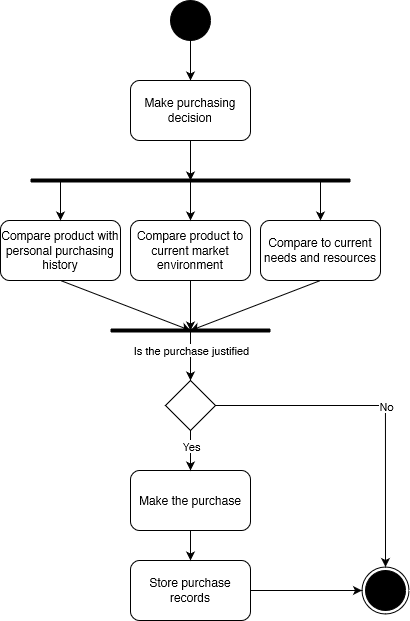
\includegraphics[width=0.6\textwidth]{currentsituation}
    \caption{Current Situation Activity Diagram}
    \label{fig:currentsituation}
\end{figure}
\subsection{The Context of the Work}
\begin{figure}[H]
    \centering
    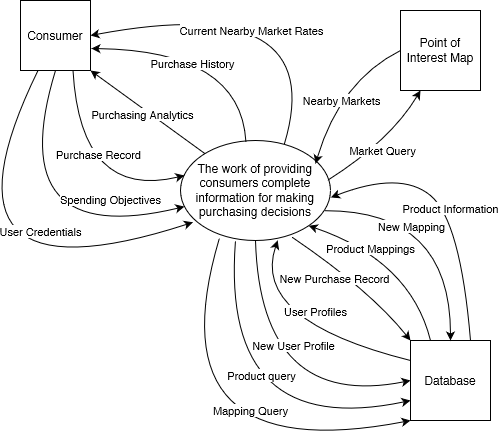
\includegraphics[width=0.9\textwidth]{workcontext}
    \caption{Work Context Model}
    \label{fig:workcontext}
\end{figure}
\subsection{Work Partitioning}
    \begin{longtable}{| >{\raggedright\arraybackslash}p{.30\textwidth} | >{\raggedright\arraybackslash}p{.30\textwidth} | >{\raggedright\arraybackslash}p{.30\textwidth} |}
        \hline
        \textbf{Event Name} & \textbf{Input/output} & \textbf{Summary of BUC} \\
        \hline
        User inputs user profile credentials & User Credentials (in) & Initialize user profile from received credentials \\
        \hline
        Consumer inputs spending objectives & Spending objectives (in) & Records the objectives and the owner \\
        \hline
        Consumer inputs purchase record & Purchase record (in) & Records the purchase and the owner of the purchase \\
        \hline
        User requests purchasing analytics & Purchasing analytics (out) & Report compiled and computed information from available data for the user profile \\
        \hline
        User requests personal purchase history & Purchase history (out) & Report compiled user purchasing history\\
        \hline
        User requests information on a product & Current nearby market rates (out) & Report market rates for a product that is accessible to the user \\
        \hline
        Compiling market information relevant to a user & Nearby markets (in) & Record information for accessible markets based on criteria \\
        \hline
        Request information on markets & Market query (out) & Send request for market information under a set of specified parameters \\
        \hline
        Database transmits product information & Product information (out) & Record information on product \\
        \hline
        New mapping received & Mapping Data (out) & Send new good/service mapping to database \\
        \hline
        Database transmits requested mapping data & Product mappings (in) & Record the product mappings \\
        \hline
        Send purchase record to database & New purchase record (out) &  Send purchase record to database \\
        \hline
        Database transmits requested user profile data & User profiles (in) &  Record the user profile data \\
        \hline
        Send user profile data & New user profile (out) &  Send a user profile to database \\
        \hline
        Send product query to database & Product query (out) & Request relevant data based on product query from database \\
        \hline
        Send mapping query to database  & Mapping query (out) &  Request relevant data based on mapping query from database \\
        \hline 
        \caption{Business Event List}
        \label{tab:businesseventlist}
    \end{longtable}
\subsection{Specifying a Business Use Case (BUC)}
\textbf{Title:} Create a new profile\\
\textbf{Trigger:} User creates a new profile\\
\textbf{Pre-condition:} User has application running\\
\textbf{Outcome: } 
\begin{enumerate}
    \item User creates an profile identified by a username and a password
    \item System creates new profile entry in database
\end{enumerate}
\textbf{Title:} Log in to user profile\\
\textbf{Trigger:} User submits profile credentials \\
\textbf{Pre-condition:} Profile exists in database \\
\textbf{Outcome: } 
\begin{enumerate}
    \item System checks if profile credentials exists
    \item If exists, system allows loads user profile
    \item If not exists, systems shows error message
\end{enumerate}
\textbf{Title:} Record user objectives \\
\textbf{Trigger:} User submits personal objectives \\
\textbf{Pre-condition:} User is logged into profile \\
\textbf{Outcome: } 
\begin{enumerate}
    \item System stores user budgeting objectives of budget with associated product or product groups
\end{enumerate}
\textbf{Title:} Input purchase records \\
\textbf{Trigger:} User submits image or manual entry of purchase record \\
\textbf{Pre-condition:} User is logged into profile \\
\textbf{Outcome: } 
\begin{enumerate}
    \item System reads and translates records to Strings
    \item System maps input records to database objects
    \item If mapping does not exist, make guesses and prompt user for feedback
    \item Save records to database
\end{enumerate}
\textbf{Title:} Create new mapping feedback \\
\textbf{Trigger:} Product mapping is not found in database \\
\textbf{Pre-condition:} Product record has been submitted \\
\textbf{Outcome: } 
\begin{enumerate}
    \item Create mapping guesses using language model
    \item Prompt user with guesses for feedback
    \item User inputs feedback
    \item Process and screen user feedback
    \item If mapping is eligible, create new mapping entry in database
\end{enumerate}
\textbf{Title:} Create user profile analytics \\
\textbf{Trigger:} User requests purchasing analytics \\
\textbf{Pre-condition:} User is logged into profile \\
\textbf{Outcome: } 
\begin{enumerate}
    \item Retrieve user data from database
    \item Transform user profile data into graphics
    \item Display graphics in application
\end{enumerate}
\textbf{Title:} Retrieve profile purchase history \\
\textbf{Trigger:} User requests purchase history\\
\textbf{Pre-condition:} User is logged into profile\\
\textbf{Outcome: } 
\begin{enumerate}
    \item Retrieve user purchase history from database
    \item Transform user purchase history into graphics
    \item Display graphics in application
\end{enumerate}
\textbf{Title:} Retrieve product information \\
\textbf{Trigger:} User requests product information\\
\textbf{Pre-condition:} User is logged into profile and has current location information set \\
\textbf{Outcome: } 
\begin{enumerate}
    \item Retrieve user purchase history from database relevant to the product
    \item Retrieve markets accessible to the user from map service
    \item Retrieve product information belonging to the accessible markets from database
    \item Transform data into graphics
    \item Display graphics in application
\end{enumerate}
\textbf{Title:} Set location information \\
\textbf{Trigger:} User sets location information \\
\textbf{Pre-condition:} User is logged into profile and location information is available \\
\textbf{Outcome: } 
\begin{enumerate}
    \item User sets initial location
    \item User sets accessibility radius
    \item Information is stored locally on device
\end{enumerate}

\section{Business Data Model and Data Dictionary}
\subsection{Business Data Model}
\begin{figure}[H]
    \centering
    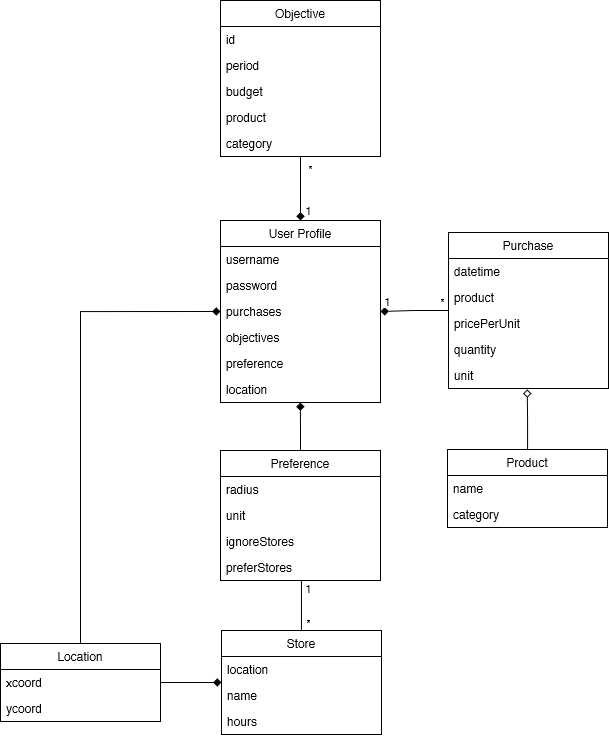
\includegraphics[width=0.85\textwidth]{classdiagram}
    \caption{Class Diagram}
    \label{fig:classdiagram}
\end{figure}
\subsection{Data Dictionary}
\begin{longtable}{| >{\raggedright\arraybackslash}p{.20\textwidth} | >{\raggedright\arraybackslash}p{.55\textwidth} | >{\raggedright\arraybackslash}p{.15\textwidth} |}
        \hline
        \textbf{Name} & \textbf{Content} & \textbf{Type} \\
        \hline
        User Profile & Username + Password + Purchases + Objectives + User Preference + User Location & Class \\
        \hline
        Objective & Objective Id + Period + Budget + Target Product + Target Category & Class \\
        \hline
        Purchase & Datetime + Purchased Product + Price Per Unit + Quantity + Unit & Class \\
        \hline
        Product & Product Name + Category & Class \\
        \hline
        Preference & Accessible Radius + Ignore Stores + Prefer Stores + Prefer Units & Class \\
        \hline
        Store & Store Location + Store Name & Class \\
        \hline
        Location & X-Coordinate + Y-Coordinate & Class \\
        \hline
        Username & *Unique String* & Attribute\\
        \hline
        Password & *String* & Attribute \\
        \hline
        Purchases & *List of Purchase class* & Attribute \\
        \hline
        Objectives & *List of Objective class* & Attribute \\
        \hline
        User Preference & *Preference class* & Attribute \\
        \hline
        User Location & *Location class* & Attribute \\
        \hline
        Objective Id & *String* & Attribute \\
        \hline
        Period & *String: day/week/month/year* & Attribute\\
        \hline
        Budget & *Currency amount measured by Double to 2 decimals* & Attribute \\
        \hline
        Target Product & *String product name* & Attribute \\
        \hline 
        Target Category & *String category name* & Attribute \\
        \hline 
        Datetime & *YYYY-MM-DD HH:MM:SS* & Attribute \\
        \hline 
        Purchased Product & *String Product name* & Attribute \\
        \hline 
        Price Per Unit & *Int price per unit of product* & Attribute \\
        \hline 
        Unit & *String* & Attribute \\
        \hline 
        Quantity & *Double* & Attribute \\
        \hline 
        Product Name & *String* & Attribute \\
        \hline 
        Category & *String* & Attribute \\
        \hline 
        Accessible Radius & *Integer* & Attribute \\
        \hline 
        Ignore Stores & *List of Stores to ignore* & Attribute \\
        \hline 
        Prefer Stores & *List of Stores to prioritize* & Attribute \\
        \hline 
        Prefer Units & *String: metric/imperial* & Attribute \\
        \hline
        Store Location & *Location class* & Attribute \\
        \hline 
        Store Name & *String* & Attribute \\
        \hline 
        X Coordinate & *Double* & Attribute \\
        \hline 
        Y Coordinate & *Double* & Attribute \\
        \hline 
        \caption{Business Event List}
        \label{tab:businesseventlist}
    \end{longtable}

\section{The Scope of the Product}

This section will go over the scope of the application being developed. It will go over the product boundary
as well as the use cases that will be considered for the product.

\subsection{Product Boundary}
\begin{figure}[H]
  \centering
  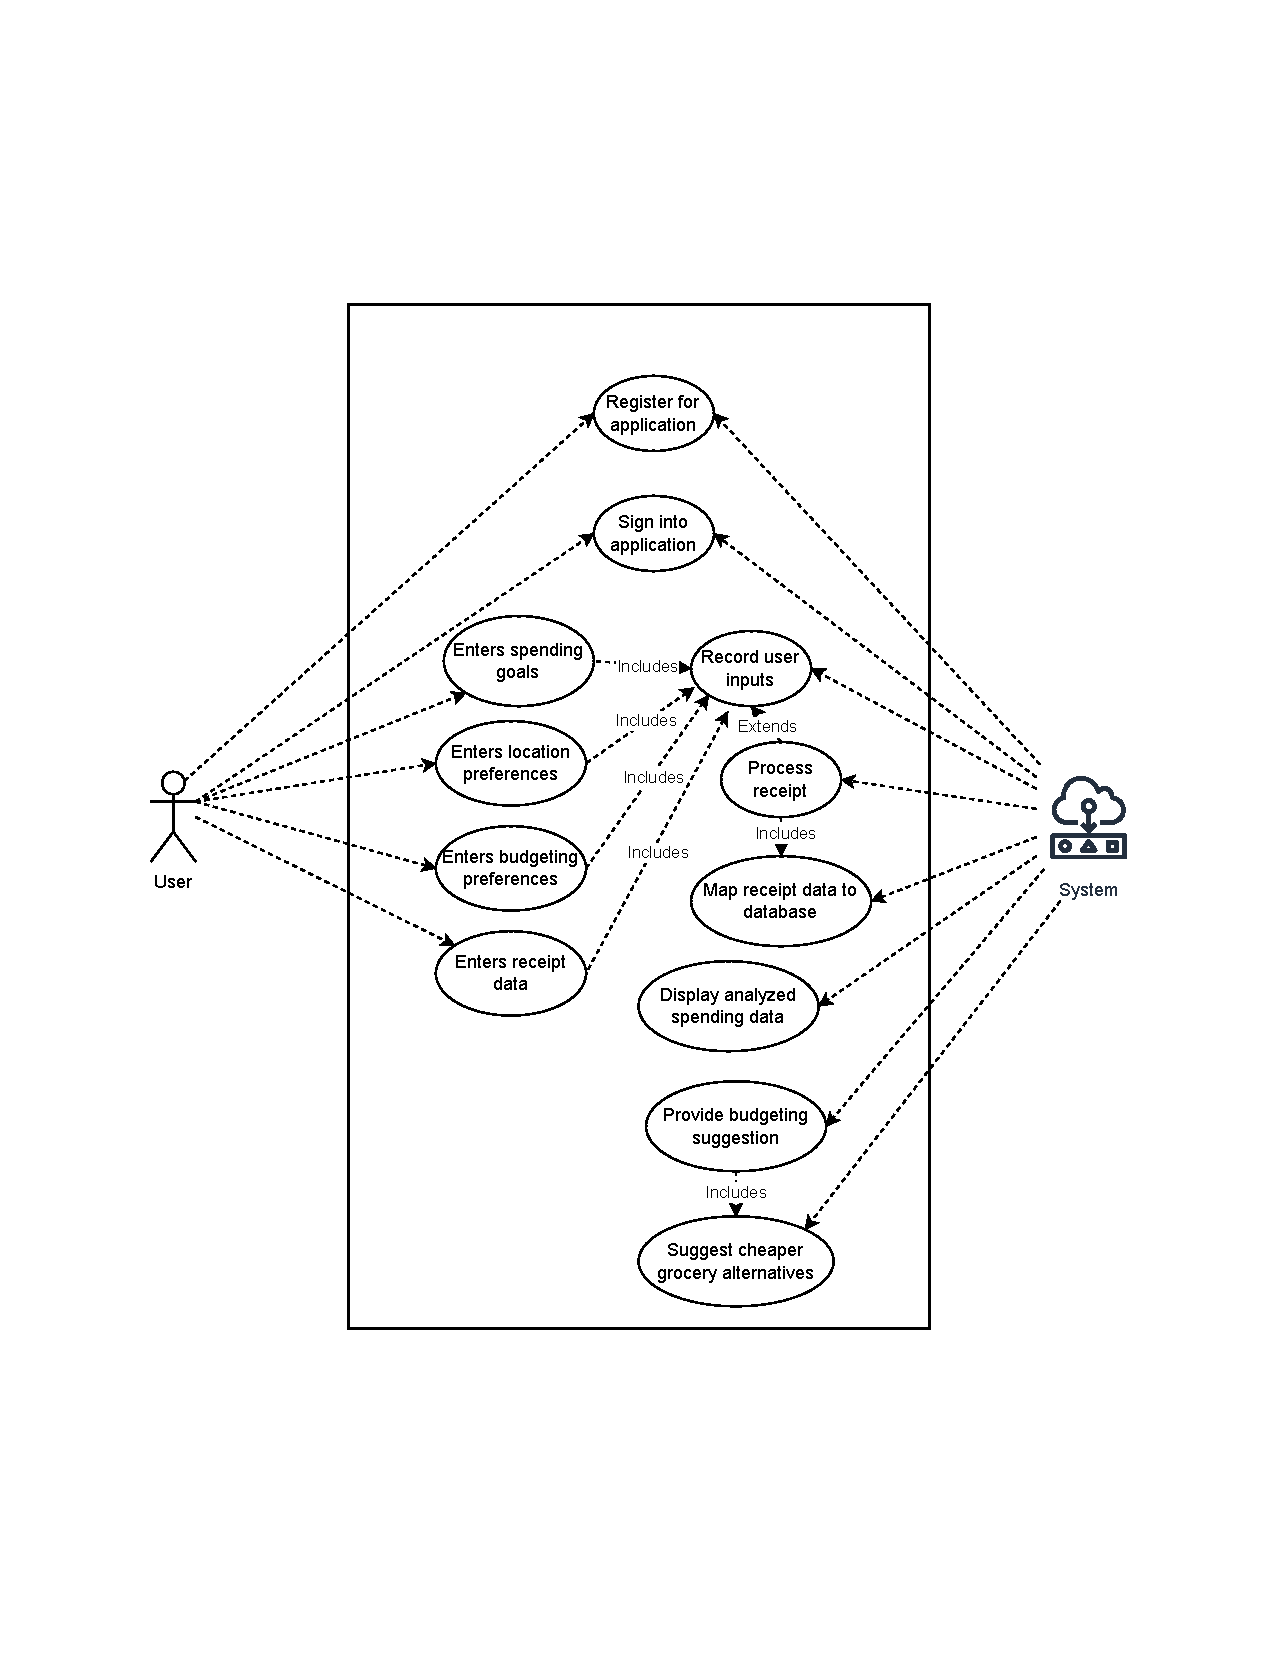
\includegraphics[width=0.95\textwidth]{use_case_diagram.pdf}
  \caption{Use Case Diagram}
  \label{fig:use_case_diagram}
\end{figure}

\pagebreak
\subsection{Product Use Case Table}

\begin{table}[H]
  \centering
  \begin{tabular}{ |c|p{3.5cm}|c|p{3.5cm}| } 
  \hline
  \textbf{PUC No} & \textbf{PUC Name} & \textbf{Actor/s} & \textbf{Input/Output} \\ 
  \hline
  1 & Register for an account & User, System & User account data (in), Created user account (out) \\
  \hline
  2 & Sign into application & User, System & User account data (in), Sign in authentication (out) \\
  \hline
  3 & Enter spending goals & User & User spending preferences (in) \\
  \hline
  4 & Enter location preferences & User & User location preferences (in) \\
  \hline
  5 & Enter budgeting preferences & User & User budgeting preferences (in) \\
  \hline
  6 & Enter receipt data & User & Photo of receipt (in) \\
  \hline
  7 & Record user inputs & System & Inputs stored in database (out) \\
  \hline
  8 & Process receipt & System & Receipt data stored in database (out) \\
  \hline
  9 & Map receipt data to database & System & Individual product data properly stored in database (out) \\
  \hline
  10 & Display analyzed spending data & System & Visualized spending data (out) \\
  \hline
  11 & Provide budgeting suggestion & System & Budgeting suggestion (out) \\
  \hline
  12 & Suggest cheaper grocery alternatives & System & Item, price, and location of cheaper alternative (out) \\
  \hline
  \end{tabular}
  \caption{Product Use Case Table}
  \label{tab:productusecasetable}
\end{table}

\pagebreak
\subsection{Individual Product Use Cases (PUC's)}

\subsubsection{Product Use Case \#1}

\textbf{Title:} Register for an account\\
\textbf{Trigger:} User wants to create an account for the application\\
\textbf{Pre-condition:} User has necessary information requested by the system\\
\textbf{Outcome:}
\begin{enumerate}
  \item User enters their email and password when prompted and submits the data.
  \item System validates the data.
  \item If valid, system stores user data in the database and creates the account.
  \item If invalid, system prompts user with an error.
\end{enumerate}

\medskip
\subsubsection{Product Use Case \#2}

\noindent \textbf{Title:} Sign into application\\
\textbf{Trigger:} User wants to sign into their account\\
\textbf{Pre-condition:} User has an account for the application\\
\textbf{Outcome:}
\begin{enumerate}
  \item User enters their email and password when prompted and submits the data.
  \item System looks for any accounts with matching credentials.
  \item If a match is found, system authentication is successful and user is granted application access.
  \item If no match is found, system authentication fails and user is prompted with an error.
\end{enumerate}

\medskip
\subsubsection{Product Use Case \#3}

\noindent \textbf{Title:} Enter spending goals\\
\textbf{Trigger:} User wants to enter their spending goals for the application\\
\textbf{Pre-condition:} User is signed into an account\\
\textbf{Outcome:}
\begin{enumerate}
  \item User enters information regarding their spending objectives and outcomes for application.
  \item System records the entered spending goals into the database.
\end{enumerate}

\medskip
\subsubsection{Product Use Case \#4}

\noindent \textbf{Title:} Enter location preferences\\
\textbf{Trigger:} User wants to enter their location preferences for the application to consider\\
\textbf{Pre-condition:} User is signed into an account\\
\textbf{Outcome:}
\begin{enumerate}
  \item User enters information regarding their current location and preferred area of coverage for the app.
  \item User selects stores they prefer and stores they want to ignore.
  \item System records the entered location preferences into the database.
\end{enumerate}

\medskip
\subsubsection{Product Use Case \#5}

\noindent \textbf{Title:} Enter budgeting preferences\\
\textbf{Trigger:} User wants to enter their budgeting preferences for the application to consider\\
\textbf{Pre-condition:} User is signed into an account\\
\textbf{Outcome:}
\begin{enumerate}
  \item User enters price range and budgeting preferences for the application to consider.
  \item System records the entered budgeting preferences into the database.
\end{enumerate}

\medskip
\subsubsection{Product Use Case \#6}

\noindent \textbf{Title:} Enter receipt data\\
\textbf{Trigger:} User wants to enter a receipt to add new spending data\\
\textbf{Pre-condition:} User is signed into an account and has a receipt to use\\
\textbf{Outcome:}
\begin{enumerate}
  \item User takes a photo of the receipt.
  \item System processes data from the receipt \textit{(see Individual Product
  Use Case for "Process receipt")} and stores data in the database \textit{(see Individual
  Product Use Case for "Map receipt data to database")}.
\end{enumerate}

\medskip
\subsubsection{Product Use Case \#8}

\noindent \textbf{Title:} Process receipt\\
\textbf{Trigger:} User enters a photo of a receipt to be analyzed by the application\\
\textbf{Pre-condition:} The receipt photo has already been taken and submitted to the application\\
\textbf{Outcome:}
\begin{enumerate}
  \item System searches the receipt looking for purchase date, time, and location information.
  \item System searches for products purchased and their prices.
  \item Products are mapped \textit{(see Individual Product Use Case for "Map receipt
  data to database")} and purchase data is recorded in the database.
\end{enumerate}

\medskip
\subsubsection{Product Use Case \#9}

\noindent \textbf{Title:} Map receipt data to database\\
\textbf{Trigger:} User enters a photo of a receipt to be analyzed by the application\\
\textbf{Pre-condition:} The receipt has already been processed by the system\\
\textbf{Outcome:}
\begin{enumerate}
  \item System goes through each found product on the receipt and
  checks if it exists in the database.
  \item If an entry in the database exists for the product, the date, time, location,
  and purchase price are recorded in that entry.
  \item If no entry for the product exists in the database, an entry is created and the
  date, time, location, and purchase price are recorded.
\end{enumerate}

\medskip
\subsubsection{Product Use Case \#10}

\noindent \textbf{Title:} Display analyzed spending data\\
\textbf{Trigger:} User wants to check their spending data\\
\textbf{Pre-condition:} The user is logged in and has spending data already entered into the application\\
\textbf{Outcome:}
\begin{enumerate}
  \item The system checks the user's purchases in the database.
  \item The system displays a visual representation of the user's purchase history and
  data is provided on what was purchased and when.
\end{enumerate}

\medskip
\subsubsection{Product Use Case \#11}

\noindent \textbf{Title:} Provide budgeting suggestion\\
\textbf{Trigger:} User exceeds budgeting preferences submitted\\
\textbf{Pre-condition:} The user is logged in and has entered their budgeting preferences into the application\\
\textbf{Outcome:}
\begin{enumerate}
  \item The system analyzes purchase history and compares it to the user's
  budgeting preferences
  \item The system suggests items to stop purchasing and/or cheaper grocery alternatives
  if they exist \textit{(see Individual Product Use Case for "Suggest cheaper grocery
  alternatives")}.
\end{enumerate}

\medskip
\subsubsection{Product Use Case \#12}

\noindent \textbf{Title:} Suggest cheaper grocery alternatives\\
\textbf{Trigger:} A recently purchased item by the user is purchased at a cheaper price\\
\textbf{Pre-condition:} A database entry for the recently purchased item and spending data exist\\
\textbf{Outcome:}
\begin{enumerate}
  \item The system analyzes recent purchase history of the item and purchase location from different users.
  \item If the location is within the current user's location preferences, the item, price and location are
  prompted to the user.
  \item If the location is not within the current user's location preferences, no prompt is created.
\end{enumerate}

\section{Functional Requirements}

This section will provide details on all the functional requirements relevant to the application.
It will also show the traceability between functional requirements and product use cases in addition to
formal specifications for some of the requirements.

\subsection{Functional Requirements}
\medskip
\noindent \textbf{Requirement ID:} FR1\\
\textbf{Use Case:} 1\\
\textbf{Description:} The system must minimize user effort and reduce the likelihood of user abandonment during registration by allowing easy access and controls to user registration.\\
\textbf{Rationale:} A registration interface is crucial for reducing the entry barrier for new users, enhancing user satisfaction, and decreasing the likelihood of registration abandonment.\\
\textbf{Fit Criterion:} The interface should allow users to enter their email and password and complete the registration in no more than three steps, with each step clearly delineated.\\

\medskip
\noindent \textbf{Requirement ID:} FR2\\
\textbf{Use Case:} 2\\
\textbf{Description:} The system must validate user credentials (email and password) when a user attempts to sign in.\\
\textbf{Rationale:}  Secure and reliable authentication is essential for protecting user accounts and sensitive data from unauthorized access and complying with data protection regulations.\\
\textbf{Fit Criterion:} Users with valid credentials must be granted access to the application, while users with invalid credentials must be denied access and receive a clear, non-ambiguous error message regarding the specific authentication failure within 3 seconds of their attempt.\\

\medskip
\noindent \textbf{Requirement ID:} FR3\\
\textbf{Use Case:} 6, 7, 8, 9\\
\textbf{Description:} The system must support the scanning and recognition of receipt data from photo images. The system must accurately recognize, extract, and parse text and numerical data from various receipt formats and layouts.\\
\textbf{Rationale:} Enabling users to upload photo images of receipts and converting these into digital spending data significantly enhances user convenience by eliminating manually entering data.\\
\textbf{Fit Criterion:} The system must successfully recognize and extract data from uploaded receipt photos with an accuracy rate over 90\% under typical lighting conditions.\\

\medskip
\noindent \textbf{Requirement ID:} FR4\\
\textbf{Use Case:} 4, 7\\
\textbf{Description:} The system must offer an interface that allows users to specify and update their current physical location and set a desired radius for area coverage.\\
\textbf{Rationale:} Enabling users to input and adjust their location and area of coverage is vital for providing customized and relevant information, services, or offers specific to their locale.\\
\textbf{Fit Criterion:} Users must be able to set and update their location and preferred area of coverage, with changes reflected in the system within 3 seconds.\\

\medskip
\noindent \textbf{Requirement ID:} FR5\\
\textbf{Use Case:} 3, 7\\
\textbf{Description:} The system must provide structured input fields where users can input and modify their grocery objectives and desired outcomes.\\
\textbf{Rationale:} Enabling users to set and alter their spending goals directly in the application allows improved grocery planning and encourages healthier grocery spending habits.\\
\textbf{Fit Criterion:} Users must be able to change their spending goals with the updated information displayed in less than a second after input.\\

\medskip
\noindent \textbf{Requirement ID:} FR6\\
\textbf{Use Case:} 5, 7\\
\textbf{Description:} The system must offer a feature where users can specify their preferred price ranges for goods and set comprehensive budgeting parameters.\\
\textbf{Rationale:} Providing users with the ability to define their price ranges and budgeting preferences is necessary for personalized shopping experience to match user constraints.\\
\textbf{Fit Criterion:} The system must reflect user's preferences in filtering and recommending products with an accuracy rate of at least 90\%.\\

\medskip
\noindent \textbf{Requirement ID:} FR7\\
\textbf{Use Case:} 8\\
\textbf{Description:} The system must process each item listed on a receipt by identifying each item details.\\
\textbf{Rationale:} Accurately capturing detailed purchase information from receipts is important for informing users with a comprehensive overview of their grocery spending habits.\\
\textbf{Fit Criterion:} The system should accurately extract and parse grocery item details from receipts, achieving a data accuracy of at least 90\%.\\

\medskip
\noindent \textbf{Requirement ID:} FR8\\
\textbf{Use Case:} 11, 12\\
\textbf{Description:} The system must analyze the user's purchase history and compare it to the budgeting preferences the user has submitted. It must suggest actions the user can take to meet their budgeting goals.\\
\textbf{Rationale:} This functionality allows users to make informed decisions and encourages them towards making well informed grocery purchases.\\
\textbf{Fit Criterion:} Suggestions should be considered relevant and useful in user feedback surveys, with at least 70\% positive response rate.\\

\medskip
\noindent \textbf{Requirement ID:} FR9\\
\textbf{Use Case:} 12\\
\textbf{Description:} The system must actively monitor prices of items that a user has purchased within the last 10 days. When it detects that an item is available at a lower price, it should promptly notify the user.\\
\textbf{Rationale:} Notifying users about lower price alternatives on grocery items they recently purchased enlightens users about potential cost saving alternatives and emphasizes the usefulness of the application.\\
\textbf{Fit Criterion:} Notifications on lower price alternatives must be delivered to the user within 24 hours of detection.\\

\medskip
\noindent \textbf{Requirement ID:} FR10\\
\textbf{Use Case:} 10\\
\textbf{Description:} The system must fetch and display a visual representation of the user's grocery purchase history, including details on items purchased and their respective timestamps.\\
\textbf{Rationale:} Providing a visual representation of grocery purchase history converts unprocessed data into a comprehensive and easily understandable format for users.\\
\textbf{Fit Criterion:} The system should present the user's purchase history data with over 95\% accuracy.\\

\medskip
\noindent \textbf{Requirement ID:} FR11\\
\textbf{Use Case:} 6, 7, 8, 9\\
\textbf{Description:} The system must allow users to verify and edit grocery items that were not accurately scanned and recognized by the system.\\
\textbf{Rationale:} It is essential for the system to ensure data accuracy and completeness of tracking of user grocery purchases. Although scanning and recognizing image text using OCR have become advanced, it is impossible to ensure 100\% accuracy of results all the time. Therefore, allowing users to verify and update items will enhance reliability of data.\\
\textbf{Fit Criterion:} The system should reflect changes made by users on the purchase items log in less than 3 seconds. Also, user feedback on ease of edit functions should be positive, with more than 80\% of users rating it easy.\\

\medskip
\noindent \textbf{Requirement ID:} FR12\\
\textbf{Use Case:} 8, 9\\
\textbf{Description:} The system must update the user's spending log in the database.\\
\textbf{Rationale:} This process enhances the management of user's grocery spending data. Additionally, the process enhances the accuracy of financial records and provides a seamless experience in tracking daily expenditures.\\
\textbf{Fit Criterion:} Upon successful extraction of data from the grocery receipt, the system should update the user's spending log in the database within 5 seconds.\\

\newpage
\begin{landscape}
  \subsection{Traceability Between Functional Requirements and Product Use Cases}

  \begin{longtable}{|l|ccccccccccc|}
		\caption{Traceability Between Functional System Test Cases and Functional Requirements} \\
		\hline
    \textbf{Functional Requirement ID}   & \multicolumn{11}{c|}{\textbf{Product Use Case ID}} \\
    \hline
    ~ & \textbf{FR1} & \textbf{FR2} & \textbf{FR3} & \textbf{FR4} & \textbf{FR5} & \textbf{FR6} & \textbf{FR7} & \textbf{FR8} & \textbf{FR9} & \textbf{FR10} & \textbf{FR11} \\
    \hline
    PUC1 & X & ~ & ~ & ~ & ~ & ~ & ~ & ~ & ~ & ~ & ~ \\
    PUC2 & ~ & X & ~ & ~ & ~ & ~ & ~ & ~ & ~ & ~ & ~ \\
    PUC3 & ~ & ~ & ~ & ~ & X & ~ & ~ & ~ & ~ & ~ & ~ \\
    PUC4 & ~ & ~ & ~ & X & ~ & ~ & ~ & ~ & ~ & ~ & ~ \\
    PUC5 & ~ & ~ & ~ & ~ & ~ & X & ~ & ~ & ~ & ~ & ~ \\
    PUC6 & ~ & ~ & X & ~ & ~ & ~ & ~ & ~ & ~ & ~ & X \\
    PUC7 & ~ & ~ & X & X & X & X & ~ & ~ & ~ & ~ & X \\
    PUC8 & ~ & ~ & X & ~ & ~ & ~ & X & ~ & ~ & ~ & X \\
    PUC9 & ~ & ~ & X & ~ & ~ & ~ & X & ~ & ~ & ~ & X \\
    PUC10 & ~ & ~ & ~ & ~ & ~ & ~ & ~ & ~ & ~ & X & ~ \\
    PUC11 & ~ & ~ & ~ & ~ & ~ & ~ & ~ & X & ~ & ~ & ~ \\
    PUC12 & ~ & X & ~ & ~ & ~ & ~ & ~ & X & X & ~ & ~ \\
    \hline
  \end{longtable}
\end{landscape}

\subsection{Added Section - Formal Specification}
In regards to identifying functions for project:
\begin{itemize}
    \item \textbf{User must provide data to application.}\\
    For all users `a' who are regular users:
    \[
    \begin{split}
        \forall a \in \text{users} \quad (& a.\text{role} = \text{``user"}\\
        & \Rightarrow a.\text{inputDataToApplication}() \Rightarrow \text{true})
    \end{split}
    \]

    \item \textbf{All data must be stored in database.}\\
    For all data `d' generated or used by the application:
    \[
    \begin{split}
        \forall d \quad (d.\text{storeInDatabase}() \Rightarrow \text{true})
    \end{split}
    \]
    
    \item \textbf{All user data must be encrypted in database.}\\
    For all user data `ud' stored in the database:
    \[
    \begin{split}
        \forall ud \quad (ud.\text{encryptInDatabase}() \Rightarrow \text{true})
    \end{split}
    \]
    
\end{itemize}

\section{Look and Feel Requirements}
In this section, any references to an \textit{E\#} refers to elicitation notes in Appendix B. \textit{E\#} corresponds
to the label for the relevant question.

\subsection{Appearance Requirements}
\begin{itemize}
  \item \textbf{AR1}: The app should have a consistent colour scheme throughout as requested in \textit{E1}. This would be
  validated through an 80\% acceptance rate from stakeholder surveys.
  \item \textbf{AR2}: App icons should convey the related feature to improve intuitiveness as requested in \textit{E1}. This
  would be validated with an 85\% success rate when asking stakeholders to pair features with icon during testing.
  \item \textbf{AR3}: The user interface should avoid clutter and features should only take up 85\% at most of available screen space
  as requested in \textit{E1}.
\end{itemize}
\subsection{Style Requirements}
\begin{itemize}
  \item \textbf{SR1}: App features and options on different pages should be in consistent locations for intuitiveness as requested in \textit{E1}.
  This would be validated through an 80\% acceptance rate from stakeholder surveys.
  \item \textbf{SR2}: Features and options should be grouped based on relation to each other to improve intuitiveness with an
  80\% acceptance rate for application organization from stakeholder surveys.
  \item \textbf{SR3}: Indicators and messages should be present to convey information such as for loading or errors as requested in \textit{E3}.
\end{itemize}

\section{Usability and Humanity Requirements}
In this section, any references to an \textit{E\#} refers to elicitation notes in Appendix B. \textit{E\#} corresponds
to the label for the relevant question.

\subsection{Ease of Use Requirements}
\begin{itemize}
  \item \textbf{EUR1}: The app should save user data and state when closed in order to minimize user input.
  \item \textbf{EUR2}: The app should allow users to undo or cancel changes made.
  \item \textbf{EUR3}: Navigation options should always be available regardless of the application page as requested in \textit{E6}.
\end{itemize}
\subsection{Personalization and Internationalization Requirements}
\begin{itemize}
  \item \textbf{PIR1}: English will be supported.
  \item \textbf{PIR2}: The app should have dark and light mode colour schemes as requested in \textit{E7}.
  \item \textbf{PIR3}: The app should allow users to enable/disable external notifications as requested in \textit{E7}.
\end{itemize}
\subsection{Learning Requirements}
\begin{itemize}
  \item \textbf{LR1}: The app should have an FAQ or Help page to assist users as requested in \textit{E5}.
  \item \textbf{LR2}: The app should have a tutorial to assist users in learning the available
  features as requested in \textit{E5}.
  \item \textbf{LR3}: Users should be able to understand core functionality of the app within 15 minutes as requested in
  \textit{E4}.
\end{itemize}
\subsection{Understandability and Politeness Requirements}
\begin{itemize}
  \item \textbf{UPR1}: The app should use common language found in the English dictionary.
  \item \textbf{UPR2}: The app should use inoffensive language based on a 90\% acceptance rate from stakeholder
  surveys.
\end{itemize}
\subsection{Accessibility Requirements}
\begin{itemize}
  \item \textbf{ACR1}: The app should allow users to change text size as requested in \textit{E7}.
  \item \textbf{ACR2}: The app should have multiple colour schemes to help those with visual impairment
  as requested in \textit{E7}.
\end{itemize}

\section{Performance Requirements}
In this section, any references to an \textit{E\#} refers to elicitation notes in Appendix B. \textit{E\#} corresponds
to the label for the relevant question.

\subsection{Speed and Latency Requirements}
\begin{itemize}
  \item \textbf{SLR1}: The app should take on average 1 second to complete backend tasks and at worst should never
  exceed 12 seconds as elicited in \textit{E8}.
  \item \textbf{SLR2}: The navigation of the app should be smooth, taking no more than 1 second to render and handle page changes
  as elicited in \textit{E8}.
\end{itemize}
\subsection{Safety-Critical Requirements}
\begin{itemize}
  \item N/A
\end{itemize}
\subsection{Precision or Accuracy Requirements}
\begin{itemize}
  \item \textbf{PAR1}: The app should be able to correctly read user inputs with over 90\% accuracy as elicited
  in \textit{E10}.
  \item \textbf{PAR2}: The app should return spending data to the user with correctness over 95\% of the intended value
  as elicited in \textit{E10}.
\end{itemize}
\subsection{Robustness or Fault-Tolerance Requirements}
\begin{itemize}
  \item \textbf{RFR1}: The app should have proper error-handling against improper user input to account for
  experimentation as elicited in \textit{E6}.
\end{itemize}
\subsection{Capacity Requirements}
\begin{itemize}
  \item \textbf{CR1}: The app should take up no more than 1GB of space as elicited in \textit{E11}.
\end{itemize}
\subsection{Scalability or Extensibility Requirements}
\begin{itemize}
  \item N/A
\end{itemize}
\subsection{Longevity Requirements}
\begin{itemize}
  \item N/A
\end{itemize}

\section{Operational and Environmental Requirements}
\subsection{Expected Physical Environment}
\begin{itemize}
    \item \textbf{EPER1} The application is expected to be compatible with smart mobile devices running Android.
    \item \textbf{EPER2} The application is expected to be compatible with smart mobile devices running IOS.
    \item \textbf{EPER3} The application is expected to be compatible with tablet devices running iPadOS or Android. 
\end{itemize}
\subsection{Wider Environment Requirements}
\begin{itemize}
    \item \textbf{WER1}: The application is designed to operate on devices equipped with camera peripherals.
    \item \textbf{WER2}: The application is designed to operate on devices that have access to the internet. 
\end{itemize}
\subsection{Requirements for Interfacing with Adjacent Systems}
\begin{itemize}
    \item \textbf{IASR1}: The application shall work with iOS 16.
    \item \textbf{IASR2}: The application shall work with Android 13.
\end{itemize}
\subsection{Productization Requirements}
\begin{itemize}
    \item N/A
\end{itemize}
\subsection{Release Requirements}
\begin{itemize}
    \item \textbf{RER1}: The application shall undergo thorough testing and quality control procedures prior to each application releases and updates. The project will aim for 80\% code coverage.
    \item \textbf{RER2}: The application shall identify and resolve defects or issues prior to application releases and updates.
    \item \textbf{RER3}: The application will be subject to a Final Demonstration from March 18 to March 29 of 2024.
\end{itemize}

\section{Maintainability and Support Requirements}
\subsection{Maintenance Requirements}
\begin{itemize}
  \item \textbf{MTR1}: All back-end maintenance and upgrades should be completed between the hours of 12:00am and 5:00am.
  \item \textbf{MTR2}: Front-end maintenance should not be coupled with backend maintenance.
  \item \textbf{MTR3}: Maintenance should be able to be completed by the non-original developers.
\end{itemize}
\subsection{Supportability Requirements}
\begin{itemize}
  \item \textbf{SPR1}: Users should be able to operate and navigate the system without any additional manual or instruction.
  \item \textbf{SPR2}: There will be a function built into the system for users to report usage issues or bugs to the developers.
\end{itemize}
\subsection{Adaptability Requirements}
\begin{itemize}
  \item \textbf{APR1}: System must operate on IOS and Android Devices.
  \item \textbf{APR2}: System is intended to be used when the user is out of their home. 
\end{itemize}

\section{Security Requirements}
\subsection{Access Requirements}
\begin{itemize}
    \item \textbf{ACR1}: The application shall require acceptance of terms and services to allow access to application's database at all times. 
\end{itemize}
\subsection{Integrity Requirements}
\begin{itemize}
    \item \textbf{INR1}: The application shall ensure data integrity by using encryption mechanisms for preventing unauthorized modifications.
    \item \textbf{INR2}: The application shall be protected from actors with harmful intentions.
\end{itemize}
\subsection{Privacy Requirements}
\begin{itemize}
    \item \textbf{PRR1}: The application shall maintain  proper data anonymization and sanitation techniques.
    \item \textbf{PRR2}: The application shall require explicit user consent to collect, process, and share user data.
\end{itemize}
\subsection{Audit Requirements}
\begin{itemize}
    \item \textbf{AUR1}: The application shall maintain audit logs that capture user activities and system events which can be reviewed by authorized system administrators.
\end{itemize}
\subsection{Immunity Requirements}
\begin{itemize}
    \item N/A
\end{itemize}

\section{Cultural Requirements}
In this section, any references to an \textit{E\#} refers to elicitation notes in Appendix B. \textit{E\#} corresponds to the label for the relevant question.
\subsection{Cultural Requirements}
\begin{itemize}
    \item \textbf{CUR1:} The app should allow users to use the metric system, imperial system, or a combination of the two (Canadian) as requested in \textit{E12} to accommodate a diverse user base and regional preferences.
    \item \textbf{CUR2:} The app should have full functionality for uncommon purchase items as requested in \textit{E12} to ensure the software is usable in the real-life dynamic market environment
    \item \textbf{CUR3:} The app should differentiate different currencies used (specifically USD and CAD) as requested in \textit{E12} to accommodate regional preferences.
\end{itemize}

\section{Compliance Requirements}
\subsection{Legal Requirements}
\begin{itemize}
    \item \textbf{LR1:} The app should comply with the app distribution platform guidelines: Google Play Store for Android, App Store for iOS
    \item \textbf{LR2:} The app should comply with local privacy laws (PIPEDA for Canada) [3]
\end{itemize}
\subsection{Standards Compliance Requirements}
N/A

\section{Open Issues}
There are currently no open issues for this project.

\section{Off-the-Shelf Solutions}
\subsection{Ready-Made Products}
There exists some existing products that address the problem we are also addressing. \\

\href{https://www.flashfood.com/}{flashfood} matches users with food that is nearing their expiration and are marked down to prevent waste and provide cheaper prices.\\

\href{https://home.ibotta.com/}{ibotta} helps users track their spending and offer coupons to those wanting to save money.\\

\subsection{Reusable Components}
\begin{itemize}
  \item \textbf{node-tesseract-ocr}: for reading labels or receipts.
  \item \textbf{PostgreSQL}: for storing relational data.
  \item \textbf{flutter}: framework for mobile app development.
\end{itemize}

\subsection{Products That Can Be Copied}
There are no known products that can legally be copied to form a solution for this problem.

\section{New Problems}
\subsection{Effects on the Current Environment}
\begin{itemize}
    \item The introduction of the new system for analyzing user spending may require integration with existing systems or databases to ensure a seamless flow of data. Changes to data connectors and interfaces may be necessary as a result, which could have an impact on the current environment.
    \item Depending on the number of users and the volume of data processed, there may be an increased network load on the current environment. Network performance may be impacted, necessitating capacity scaling.
\end{itemize}
\subsection{Effects on the Installed Systems}
\begin{itemize}
    \item The new system should be compatible with the operating systems, browsers, and hardware configurations used by existing users. Compatibility problems could cause system outages or user access problems.
    \item Integration with existing security systems is important to ensure that user data remains secure. Data breaches or unauthorised access could result from any security integration flaws.
\end{itemize}
\subsection{Potential User Problems}
\begin{itemize}
    \item Users may experience difficulties adjusting to the new system, particularly if it significantly alters the user interface or process. To deal with this problem, training and support materials should be made accessible.
    \item Users might encounter problems during the migration of their existing spending data to the new system. Ensuring a smooth transition and data integrity is essential.
\end{itemize}
\subsection{Limitations in the Anticipated Implementation Environment That May
Inhibit the New Product}
\begin{itemize}
    \item The anticipated implementation environment might not entirely satisfy the new product's hardware or software requirements. This could result in system instability or reduced performance.
\end{itemize}
\subsection{Follow-Up Problems}
\begin{itemize}
    \item After the initial implementation, updates, bug fixes, and maintenance will be required. If issues are not addressed promptly, users may grow dissatisfied.
\end{itemize}

\section{Tasks}
\subsection{Project Planning}
\begin{table}[H]
  \centering
  \begin{tabular}{ |c|c| } 
  \hline
  \textbf{Deliverable} & \textbf{Deadline} \\ 
  \hline
  Hazard Analysis Revision 0 & October 20 \\
  \hline
  V\&V Plan Revision 0 & November 3 \\ 
  \hline
  Proof of Concept Demonstration & November 13-24 \\ 
  \hline
  \end{tabular}
  \caption{Development Phase 1}
  \label{tab:developmentphase1}
\end{table}

\begin{table}[H]
  \centering
  \begin{tabular}{ |c|c| } 
  \hline
  \textbf{Deliverable} & \textbf{Deadline} \\ 
  \hline
  Design Document Revision 0 & January 17 \\
  \hline
  Revision 0 Demonstration & February 5-February 16 \\ 
  \hline
  \end{tabular}
  \caption{Development Phase 2}
  \label{tab:developmentphase2}
\end{table}

\begin{table}[H]
  \centering
  \begin{tabular}{ |c|c| } 
  \hline
  \textbf{Deliverable} & \textbf{Deadline} \\ 
  \hline
  V\&V Report Revision 0 & March 6 \\ 
  \hline
  Final Demonstration (Revision 1) & March 16-March 29 \\
  \hline
  Final Documentation (Revision 1) & April 4 \\ 
  \hline
  \end{tabular}
  \caption{Development Phase 3}
  \label{tab:developmentphase3}
\end{table}
\subsection{Planning of the Development Phases}

Development is being split into three phases based on an overarching goal for each: the Proof of Concept build,
the Revision 0 build, and the Revision 1 build. \par

The first development phase has a focus on initial documentation and implementation.
Rather than building a full app at the phase, development will involve familiarization with
the technology and constructing core features to prove the concept is feasible. This phase will
end with the Proof of Concept Demonstration where the feasibility will be proven to stakeholders.
Priorities will largely be based on deadlines and will largely follow the set deadlines by the
course instructor. As shown below, moving forward, documentation will take priority while
development for the Proof of Concept build occurs concurrently. In other words, writing the
the necessary documents will take priority and any spare time will be spent developing. Once
the final document deadline of this period is reached, development will be focused on until
the demo date. \par

\begin{figure}[H]
  \centering
  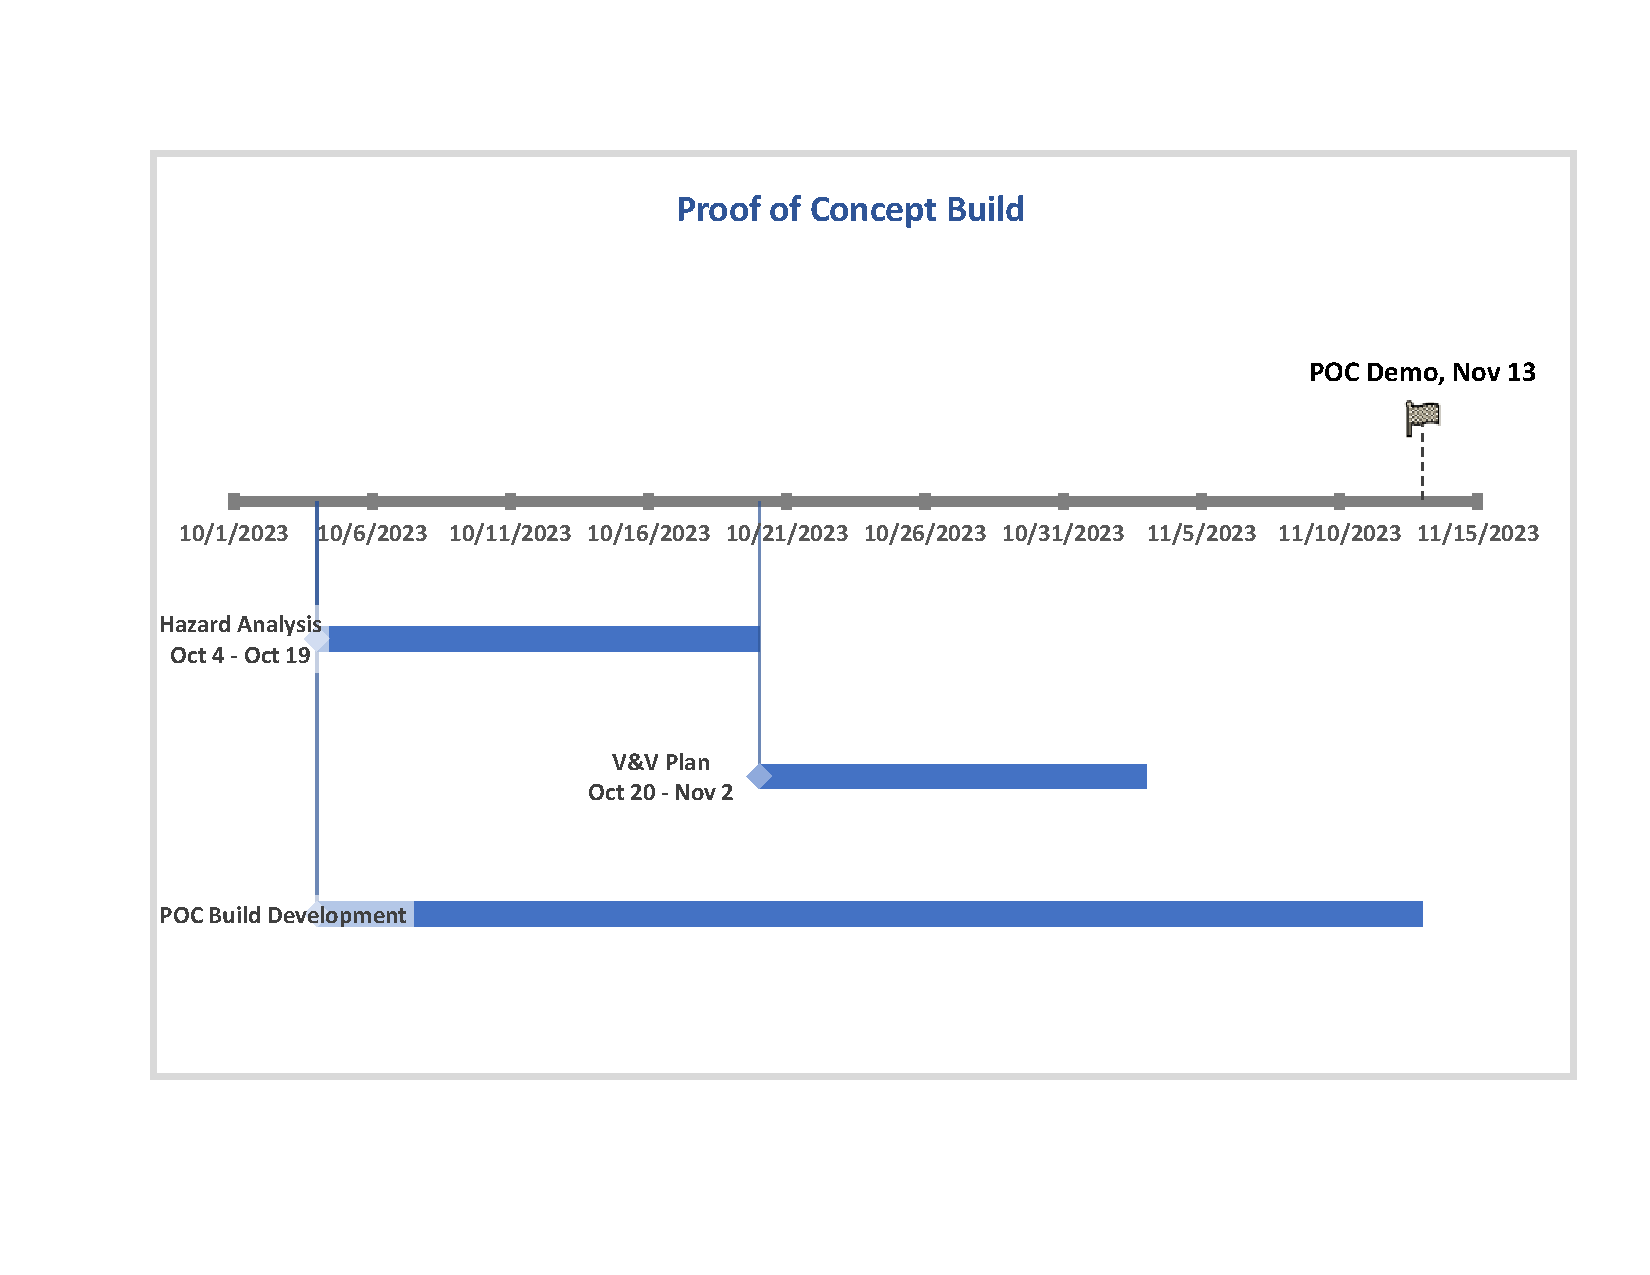
\includegraphics[width=\textwidth]{proofofconcepttimeline.pdf}
  \caption{Proof of Concept Build Timeline}
  \label{fig:ProofOfConceptTimeline}
\end{figure}

The second phase of development will focus on design of the application and constructing the
Revision 0 build of the application. With the initial functionality from the first development phase as
a starting point, the actual app structure will be built around it. This will include more UI/UX
development as well as additional features that are needed for the Revision 0 version. This phase ends
with the Revision 0 Demonstration where stakeholders can see the first iteration of the full application
and provide feedback. Priority will be given to the Revision 0 build during this phase due to most
of the documentation already being completed in the previous phase.
This will continue until January 1 where the team will shift priority to the Design Documentation due to
the earlier deadline. After completion, the team will continue working on the Revision 0 build until
the demo date on February 5. \par

\begin{figure}[H]
  \centering
  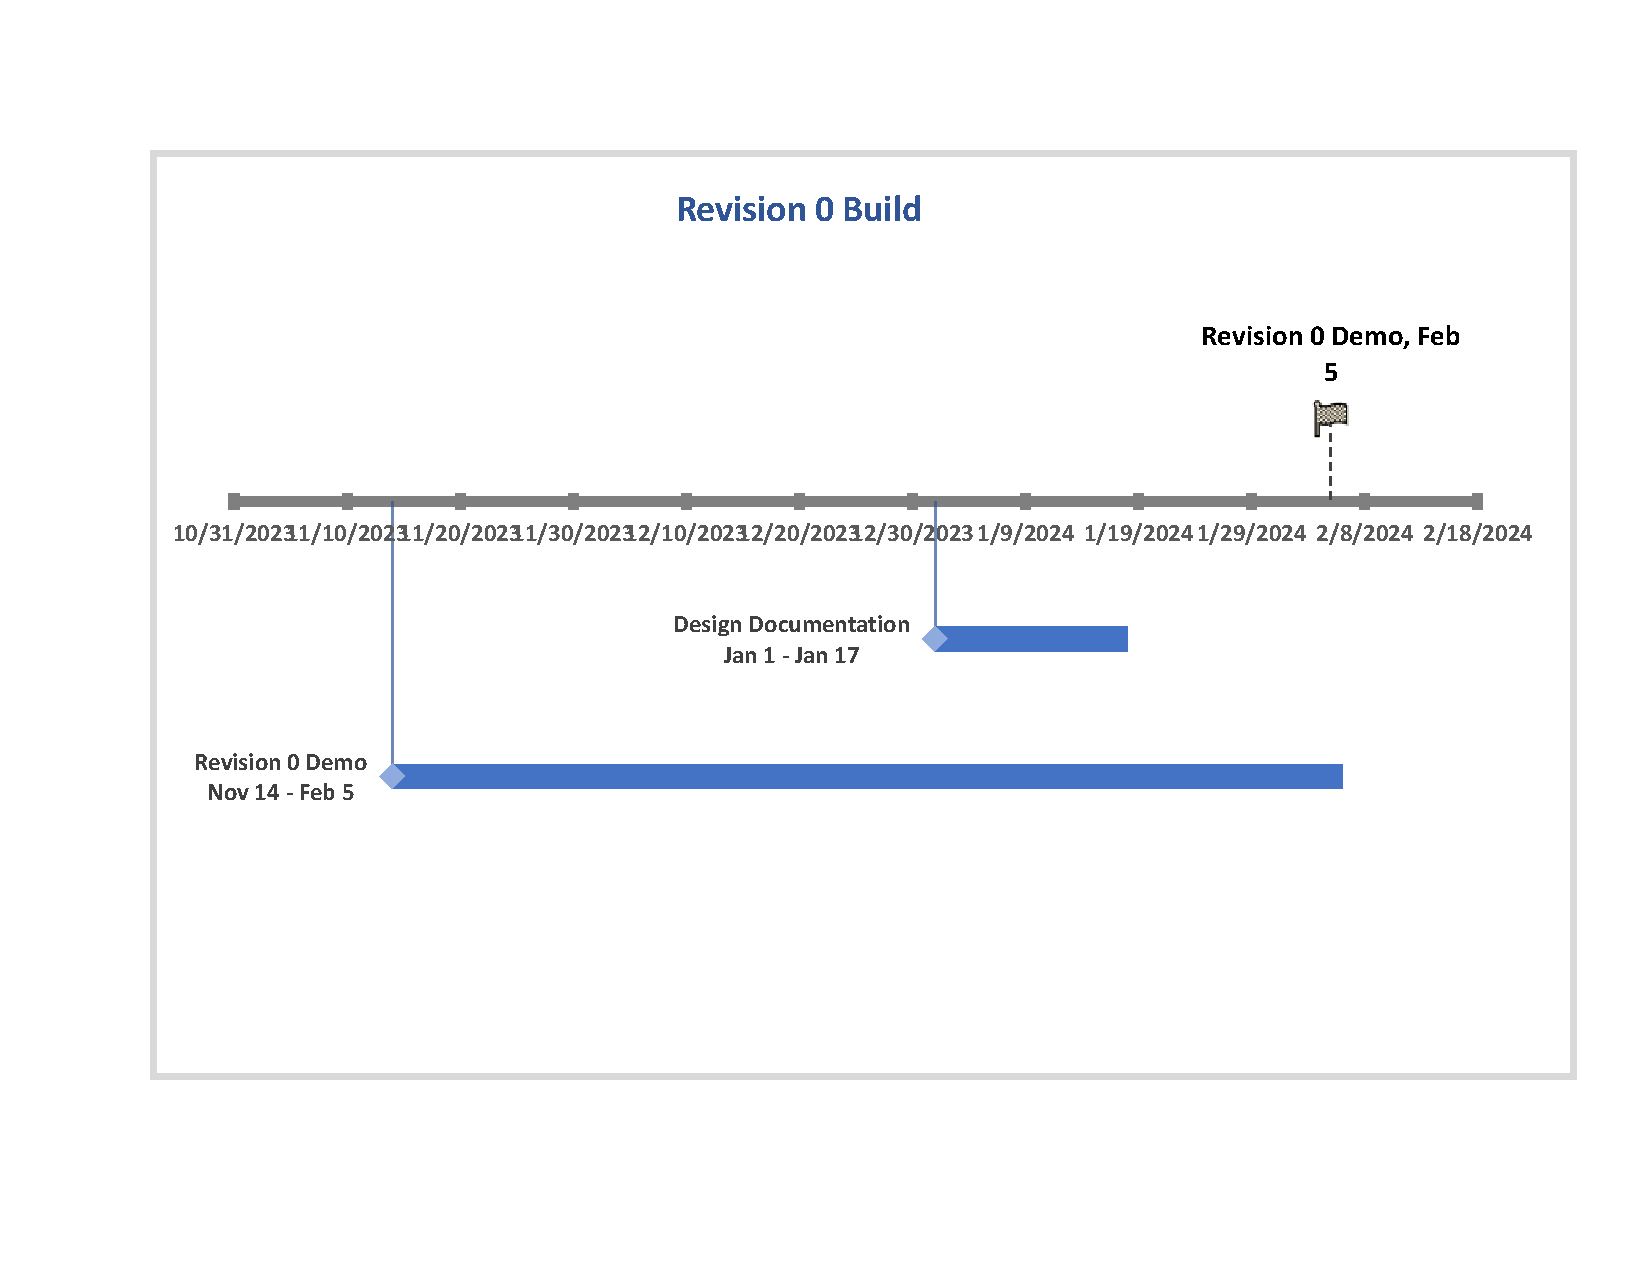
\includegraphics[width=\textwidth]{revision0timeline.pdf}
  \caption{Revision 0 Build Timeline}
  \label{fig:Revision0Timeline}
\end{figure}

The third phase of development is focused on reviewing Revision 0 and iterating on feedback from the
Revision 0 Demonstration. Here, documentation will be reviewed and finalized based on any changes made
during development. Furthermore, no new large-scale features will be implemented. Instead, development
will be restricted to improving the Revision 0 version and implementing feedback from stakeholders. This phase
will end with the Revision 1 Demonstration and submission of the finalized Revision 1 Documentation. Priority
will be first given to the V\&V Report due to it having the earliest deadline along with development for the Revision 1
build occurring concurrently at a lower priority. Once the V\&V report is completed, the Revision 1 Build will take priority
until the demo with Revision 1 Documentation occurring concurrently in March. Once the demo is completed, the team will
continue to finalize documentation until its deadline.

\begin{figure}[H]
  \centering
  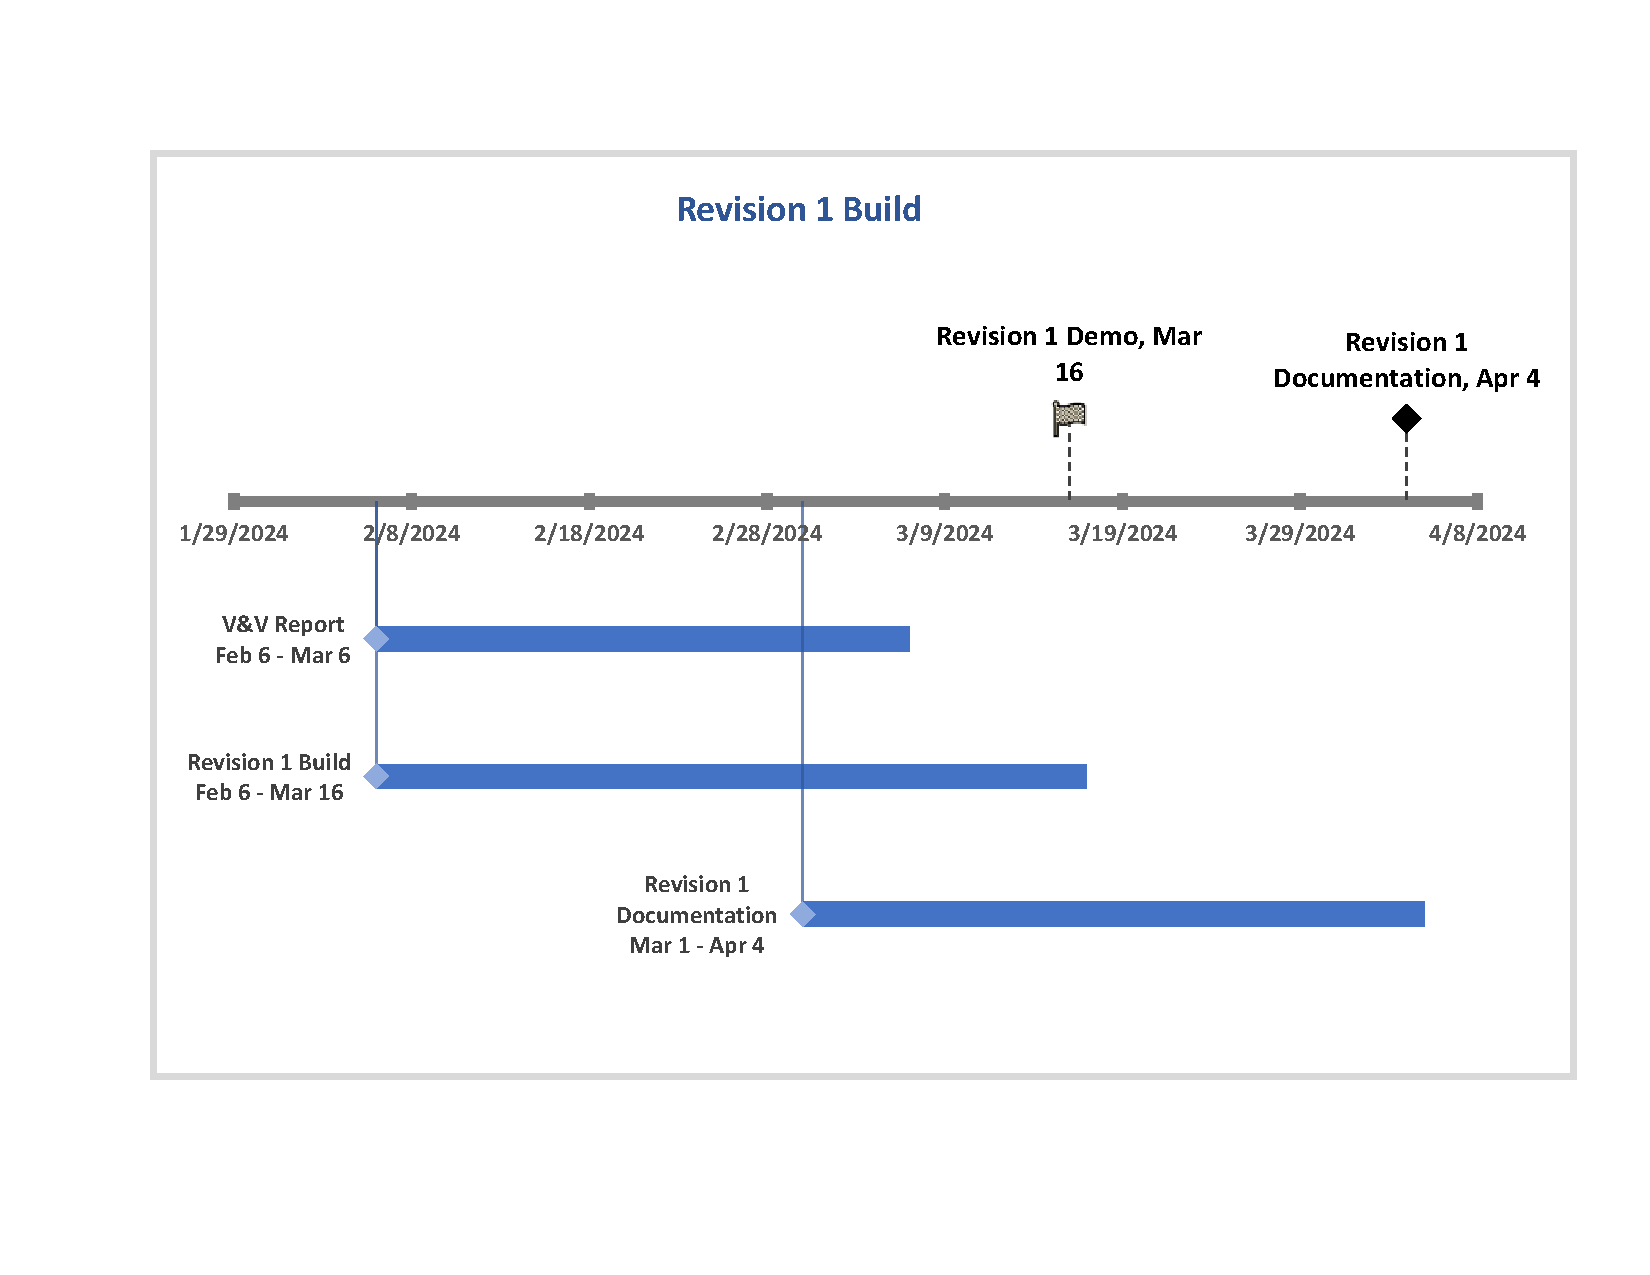
\includegraphics[width=\textwidth]{revision1timeline.pdf}
  \caption{Revision 1 Build Timeline}
  \label{fig:Revision1Timeline}
\end{figure}


\section{Migration to the New Product}
\subsection{Requirements for Migration to the New Product}
N/A
\subsection{Data That Has to be Modified or Translated for the New System}
N/A

\section{Costs}
The team currently has no intention of spending money and aims to utilize free software and technology
for this project.

\section{User Documentation and Training}
\subsection{User Documentation Requirements}
\begin{itemize}
    \item The application shall give detailed instructions on how to use the application in user manuals or guides. Registration, sign-in, data entry, budgeting, spending analysis, and any other key features should all be included in this documentation.
    \item The application shall offer a FAQ section that answers to frequent user issues and inquiries. This can enable users to quickly find answers to their problems without the need for outside assistance.
    \item The application shall offer a troubleshooting guide that details common problems and how to fix them. This should include technical difficulties, login issues, and data sync issues.
    \item The application shall inform users on how to stay up to speed with software updates and new features. Include release notes that describe the additions and modifications done in each update.
\end{itemize}
\subsection{Training Requirements}
\begin{itemize}
    \item The application shall provide on-boarding content that new users can access when they initially register for the application, such as tutorial videos or guidelines. These resources should to make it easier for users to learn the basic features.
    \item The application shall clearly communicate the available user support channels, such as a customer support email, chat, or phone number. Users should be made aware of where to look for assistance when they run into problems.
    \item The application shall provide a system that will allow users to comment on the documentation and training materials. The training procedure and documentation quality can be continually improved with the help of this feedback.
\end{itemize}

\section{Waiting Room}
At the moment, there are no requirements or features being excluded from the initial version.

\section{Ideas for Solution}
Some initial ideas for the implementation that the team came up with are as follows:
\begin{itemize}
    \item Application will utilize \textit{node-rsa} to handle encryption and security for user data.
    \item Front-end will use MVVM architecture.
    \item Natural language processing will be used to assist mapping from receipts to the database.
\end{itemize}

\newpage{}
\section*{Appendix A --- Reflection}

The information in this section will be used to evaluate the team members on the
graduate attribute of Lifelong Learning.  Please answer the following questions:

\begin{enumerate}
  \item \textbf{What knowledge and skills will the team collectively need to acquire to
  successfully complete this capstone project?  Examples of possible knowledge
  to acquire include domain specific knowledge from the domain of your
  application, or software engineering knowledge, mechatronics knowledge or
  computer science knowledge.  Skills may be related to technology, or writing,
  or presentation, or team management, etc.  You should look to identify at
  least one item for each team member.}

  For this application, many skills will be required in order to ensure this
  project's success. This includes a combination of project specific knowledge
  as well as a few less technical skills. Together, these skills will ensure the
  smooth development of our application but will also likely prove useful in the future
  as we move forward with our careers.
  \begin{enumerate}
    \item Working knowledge of \textit{Flutter} development and front-end design
    \item Knowledge working with \textit{Node.js} backends and REST APIs
    \item Skills related to the use of the \textit{Tesseract-OCR} engine
    \item Working knowledge of \textit{PostgreSQL}
    \item Experience working with Natural Language Processing or Machine Learning
    \item Writing proper software documentation
    \item Familiarity and experience with software testing/coverage
    \item Presentation and communication skills for elicitation and demos
  \end{enumerate}  

  \item \textbf{For each of the knowledge areas and skills identified in the previous
  question, what are at least two approaches to acquiring the knowledge or
  mastering the skill?  Of the identified approaches, which will each team
  member pursue, and why did they make this choice?}

  For the above skills, there are many approaches that could be taken to learning
  and developing them. In terms of skills \textit{(a)} to \textit{(e)}, these would be categorized as
  development oriented skills. These would involve knowledge that could directly apply to
  the technology being employed for this capstone project. Since these are each popular
  technologies in their own right, many resources could be accessed to learn about them. Watching
  \textit{YouTube} videos and tutorials would be one resource that could be used to strengthen
  and learn these skills. \textit{YouTube} tutorials often provide more practical applications
  for the skill in question and the site has content that covers a wide variety of topics.
  Additionally, official documentation could be read in order to see how the original developers intend
  the technology to be used. This would provide a more in-depth understanding of each aspect of the
  technology. There are also plenty of third-party online articles and forums that could be referenced when
  learning these types of skills. One last approach that could be taken is referencing open-source
  projects using these technologies to see how they are used in real development.\par

  Skills \textit{(f)} and \textit{(g)} are technical but less directly involved with the coding portion
  of development. Despite this, there are still plenty of resources that could be used to learn and
  familiarize ourselves with them. One place to look could be previous coursework, in particular,
  \textit{SFWRENG 3RA3} and \textit{SFWRENG 3S03} notes could be used to reference documentation and
  software testing respectively. Furthermore, resources for these topics also exist on \textit{YouTube}
  which could be leveraged in addition to third-party articles. One last resource could also be to leverage
  group work and collaboration. This would provide active engagement as well as opportunity
  for feedback to improve these skills.\par

  Lastly, skill \textit{(h)} is a general skill that is important for all engineers to be comfortable
  with. One approach to mastering this skill could be practical applications, including but not limited to holding
  mock presentations or focus groups with the team. Practicing presentations and communication is one of the
  easiest ways to help develop this skill. Moreover, there are many seminars and courses online that help
  teach strong communication practices such as ones on \textit{Coursera} or \textit{LinkedIn Learning}.\par

  With these in consideration, each team member has listed their chosen skills, their chosen approaches from above,
  and why they chose to pursue these skills below.

  \textbf{Ryan Yeh}\\
  \textit{Chosen Skills: (a), (f), (g), (h)} \\
  At the beginning of this project, I was assigned as the lead for documentation and testing. As such,
  I would like to take the opportunity to strengthen my understanding of these skills in order to meet my team's
  expectations. Outside of this project though, I believe these skills will be very helpful regardless of what type
  of developer I end up becoming. Additionally, I wanted to strengthen my understanding and skills in front-end
  development. UI design is a software field that I have an interest in but lack sufficient experience currently.
  Therefore, I would love to take this opportunity to learn more about it and strengthen my understanding of it. Lastly,
  I chose communication skills as something to focus on due to my belief that it is something I could improve upon.
  Communication and presentation skills will always be universally needed and putting an emphasis on it now would greatly
  help me in the future. \par
  My approach for developing my documentation and software testing skills will be to refer to previous year course notes.
  This will help me to reinforce the material I have already learned and refresh myself on topics I may have forgotten.
  I also plan to read third-party articles as a supplement to learn more about certain
  topics that may not have been covered in as much detail in class. For \textit{Flutter} and front-end design,
  I plan to watch \textit{YouTube} tutorials in order to get more a hands-on experience with the technology. I also
  plan to reference documentation and articles in order to further my learning beyond the videos watched. Finally,
  I will leverage my group in order to strengthen my communication skills. I will try and place myself into positions
  that force me to practice communication such as leading meetings, as well as practicing presentations with the
  rest of my team.

  \medskip
  \textbf{Sawyer Tang}\\
  \textit{Chosen Skills: (a), (b), (d), (h)} \\
  For this project, I was assigned to backend development. In following this, I am choosing to improve my abilities in \textit{NodeJS} and \textit{SQL}. I have used some of these technologies in brevity over my past internship positions but I am looking to deepen my experience with them further with the hopes of bringing this experience to future personal projects and jobs. 
  In addition to wanting to improve my backend skills, I also want to dive into front end. More specifically, mobile development in \textit{Flutter}. This is something that I have always had an interest in learning and this project seems to me like a perfect opportunity.
  Finally, I believe that being able to effectively communicate your ideas is an invaluable skill and it is something that I am always looking to improve for myself and career. \par
  My approach to gaining these frontend and backend skills will be to consume public documentation, online forums, and \textit{YouTube} video tutorials. For communication skills, I practice them every day during meetings or when working with team members. I also look to improve these skills during our team presentations and demos.

  \medskip
  \textbf{Jason Nam}\\
  \textit{Chosen Skills: (a), (c), (e), (g)}\\
  During the early stages of project team formation and idea generation, I was tasked with the job of undertaking feasibility studies related to implementing OCR for the team's project solution. At that point in time, I had extensive experience working with Machine Learning for Natural Language Processing. However, I had never had the opportunity to learn proper Machine Learning models related to OCR. I am eager to learn the workings behind OCR and how we can implement it in our project. I am also eager to further enhance my ML for NLP skills.
  Similar to my previous point, I also had the opportunity to experience full-stack development involving web development. However, I never had a chance to learn Mobile App development, especially front-end app development. I am confident I can utilize my skills from web development to transfer over to app development and improve from there on.
  Finally, I want a tangible skill I can acquire during the duration of this project. I believe that skills related to software testing and coverage will be very valuable later on in life. \par
  My approach to acquiring OCR and Machine Learning Recognition skills will involve extensively reading over the user manual for \textit{Tesseract OCR} package. Fortunately, there are many sources of information related to Tesseract OCR online in many different platforms, including \textit{YouTube}, \textit{Tesseract Github Repository}, and official user manuals. For app development using \textit{Flutter}, I want to start from the fundamentals. First, I will endeavor to learn \textit{Dart} programming language, which is the programming language behind \textit{Flutter}. Then, I will refer to many open source \textit{Flutter} development projects to familiarize myself with official \textit{Flutter} development. For software testing and coverage related skills, I will refer to previous course 3S03 - Software Testing course to re-acclimatize myself on the topic.

  \medskip
  \textbf{Allan Fang}\\
  \textit{Chosen Skills: (a), (c), (f), (h)} \\
  I will be the primary developer for the frontend and OCR portions of this project. For these skills (\textit{a} and \textit{c}), I will pursue both the approach of following tutorials and the approach of reading documentation. From past experiences, I have found that there is a knowledge aspect and execution aspect to skills similar to the aforementioned. While documentation is usually very comprehensive, I feel that it is necessary to supplement the learning process with additional material. Following or just watching a tutorial of these skills in action are usually good ways to fill in the knowledge gaps. \par
  For skills \textit{f} and \textit{h} that all groups members will be responsible for, I will be pursuing the approach of practice and feedback (which also includes referring to past course work). I believe that for these skills, practical application is most important. Actively engaging in these skills, along with consistent feedback and improvement, will allow me and my group mates to develop a deeper understanding of these skills in the personal application context. Furthermore, feedback from multiple sources can introduce broader perspectives previously unknown and will result in immediate improvements.

\end{enumerate}

\section*{Added Section - Appendix B --- Stakeholder Requirements Elicitation Notes}

\begin{itemize}
  \item \textbf{E1:} Consider your favourite or most used mobile apps, what elements of the UI
  stand out? What in your opinion makes an appealing user interface?
    \begin{itemize}
      \item Minimize options to create a cleaner UI.
      \item Utilization of easily accessible menu bars (like Instagram) to improve navigation UX.
      \item Consistent and cohesive colour theme throughout.
      \item Use of icons that clearly convey what the option is meant for.
      \item Put options in consistent locations to minimize hand movements (easy to tap interface).
    \end{itemize}
  \item \textbf{E2:} When you think of intuitive applications, what about the application makes
  the UI or UX intuitive?
    \begin{itemize}
      \item Many apps borrow UI layouts from each other, helps with familiarity in terms of navigation.
      \item Always accessible navigation options.
      \item Proper organizing of features (unrelated features should be separated on the UI).
      \item Swipe navigation and minimal long presses.
      \item Saving state when closed to minimize user input on future uses.
    \end{itemize}
  \item \textbf{E3:} How important do you consider application feedback and what feedback would you
  expect from an application? (i.e. loading indicators)
    \begin{itemize}
      \item High importance to communicate errors and loading to users.
      \item Should always convey when issues happen or something is being done.
      \item When fetching information or other longer duration tasks, loading bar should be utilized.
      \item Utilization of messages or pop ups if resources are unavailable or something goes wrong.
    \end{itemize}
  \item \textbf{E4:} When learning a new app, how long would you consider a reasonable amount of time
  to consider an app easy-to-use?
    \begin{itemize}
      \item Average acceptable time to consider an app intuitive would be to be able to figure
      out basic functionality within 15 minutes.
    \end{itemize}
  \item \textbf{E5:} What features would you want to help with the learning experience of a new app?
    \begin{itemize}
      \item The use of a tutorial on first launch to take users through the UI and different features.
      \item The use of tooltips for certain options and features.
      \item A button that users can press to access a Help menu or FAQ.
    \end{itemize}
  \item \textbf{E6:} How do you usually go about learning a new application?
    \begin{itemize}
      \item All participants said they tend to brute force applications in order to learn
      (i.e. clicking around and seeing how the application responds).
      \item As an addition to this brute force approach, participants explained how useful an
      undo feature would be as well as always accessible navigation.
    \end{itemize}
  \item \textbf{E7:} If you were using an application, what personalizations/accessibility settings
  would you consider a must?
    \begin{itemize}
      \item Dark/Light mode.
      \item Ability to  change text sizes.
      \item Multiple language support.
      \item Allowing users to enable or disable notifications if used.
      \item Alternate color palettes to help with those with visual impairment like color blindness.
    \end{itemize}
  \item \textbf{E8:} Consider an app you use often, generally, how long would you say you wait for operations
  to complete? How long would you be willing to wait for an application before closing the app?
    \begin{itemize}
      \item Ideally, regular operations should take a second or less.
      \item At most, participants would wait an average of 12 seconds before closing the app or
      thinking something went wrong.
    \end{itemize}
  \item \textbf{E9:} What kind of phone do you use? (Apple/Android/Other)
    \begin{itemize}
      \item All participants used Apple devices.
    \end{itemize}
  \item \textbf{E10:} On a scale of 1-10, for an app of this nature, how important would you consider accuracy
  of the system and data? How important would you consider responsiveness on the same scale?
    \begin{itemize}
      \item All participants considered accuracy of the features and data to be the most important (10) due
      to the financial aspect of the app.
      \item Responsiveness was considered important (8) in order to ensure a positive user experience. If the
      app does not feel good to use, most participants said they would find another app instead.
    \end{itemize}
  \item \textbf{E11:} How much do you consider the size of an application you install? How big of an app would you
  consider reasonable?
    \begin{itemize}
      \item Most participants said they did not pay much attention to the size of applications when installing
      them.
      \item Participants said they would consider anything over 1GB unreasonable for an app of this nature.
    \end{itemize}
  \item \textbf{E12:} For an app of this nature, what features or points of interest come to mind based on your identity as a Canadian?
    \begin{itemize}
      \item Participant stated imperial and metric units are hard to navigate as Canada uses a unique mix. 
      them.
      \item Participant stated that culturally unique grocery items (such as Chinese vegetables) need to be included.
      \item Participant stated that the app should consider USD vs CAD as purchases from the United States are common when living in Canada
    \end{itemize}
\end{itemize}

\section*{Added Section - Appendix C --- Bibliography}

[1] N. Barghiel, “Soaring food prices are changing the way Canadians shop for groceries - national,” Global News, \url{https://globalnews.ca/news/9857853/food-inflation-grocery-shopping-habits-canada/} (accessed Nov. 29, 2023). 

[2] [1] N. Ziafati, “Here are the food prices that increased, decreased in October,” CTVNews, \url{https://www.ctvnews.ca/canada/here-are-the-food-prices-that-increased-decreased-in-october-1.6654483#:~:text=Grocery%20inflation%20was%20at%205.4,inflation%20rate%2C%20the%20report%20showed.} (accessed Nov. 29, 2023). 

[3] Office of the Privacy Commissioner of Canada, “Seizing opportunity: Good privacy practices for developing mobile apps,” Office of the Privacy Commissioner of Canada, \url{https://www.priv.gc.ca/en/privacy-topics/technology/mobile-and-digital-devices/mobile-apps/gd_app_201210/} (accessed Oct. 4, 2023). 
\end{document}